\chapter{Conception du projet}
\minitoc
\clearpage
\section{Introduction}
Afin de créer une application respectant les besoins définis dans le cahier de charges, il faut d'abord passer par l'étape de conception. Cette étape permettra de décortiquer le cahier de charges et définir les acteurs, les cas d'utilisation, et finalement les différentes classes qui définissent les différents attributs de chaque entité qui interagit avec l'application.
\section{Spécification des besoins}
La première étape de la conception est de dégager les différents besoins de l'utilisateur. Ces besoins sont divisés en deux catégories: fonctionnels et non fonctionnels.
\subsection{Besoins fonctionnels}
\subsubsection{L'authentification}
Le client doit s'authentifier pour utiliser les différents services de l'application.
\subsubsection{Consulter les voitures disponibles}
Le client peut consulter les voitures disponibles selon sa position actuelle.
\subsubsection{Créer une réservation}
Le client peut créer un réservation en choisissant une voiture.
\subsubsection{Paiement en ligne}
Le client peut payer pour sa réservation à l'aide des méthodes de paiement en ligne.
\subsubsection{Signature numérique de contrat de location}
Le client peut signer son contrat de location en ligne en toute sécurité.
\subsubsection{Suivre la position de la voiture}
Le client peut suivre la position de la voiture louée en temps réel.
\subsubsection{Contacter le chauffeur}
Le client peut contacter le chauffeur de sa voiture louée par appel téléphonique ou messagerie instantanée.
\subsection{Besoins non fonctionnels}
\subsubsection{Interfaces graphiques}
L'utilisateur peut rapidement commencer à utiliser l'application sans difficulté à l'aide d'interfaces graphiques claires et simples.
\subsubsection{Performances de l'application}
L'application ne doit pas présenter des imperfections en termes de rapidité et de fluidité en cours de son exécution.
\subsubsection{Maintenabilité et scalabilité}
L'application doit être simple à maintenir et facilement scalable dans le futur.
\subsubsection{Sécurité}
Toutes les informations traitées dans l'application doivent êtres protégées, et une vérification de l'utilisateur est impérative avant chaque opération.
\section{Diagrammes UML}
\subsection{Diagramme de cas d'utilisation}
L'application SPN-Cars a un seul acteur qui est l'utilisateur, ce dernier utilisera toutes les fonctionnalités offertes par l'application.
\begin{figure}[H]
    \centering
    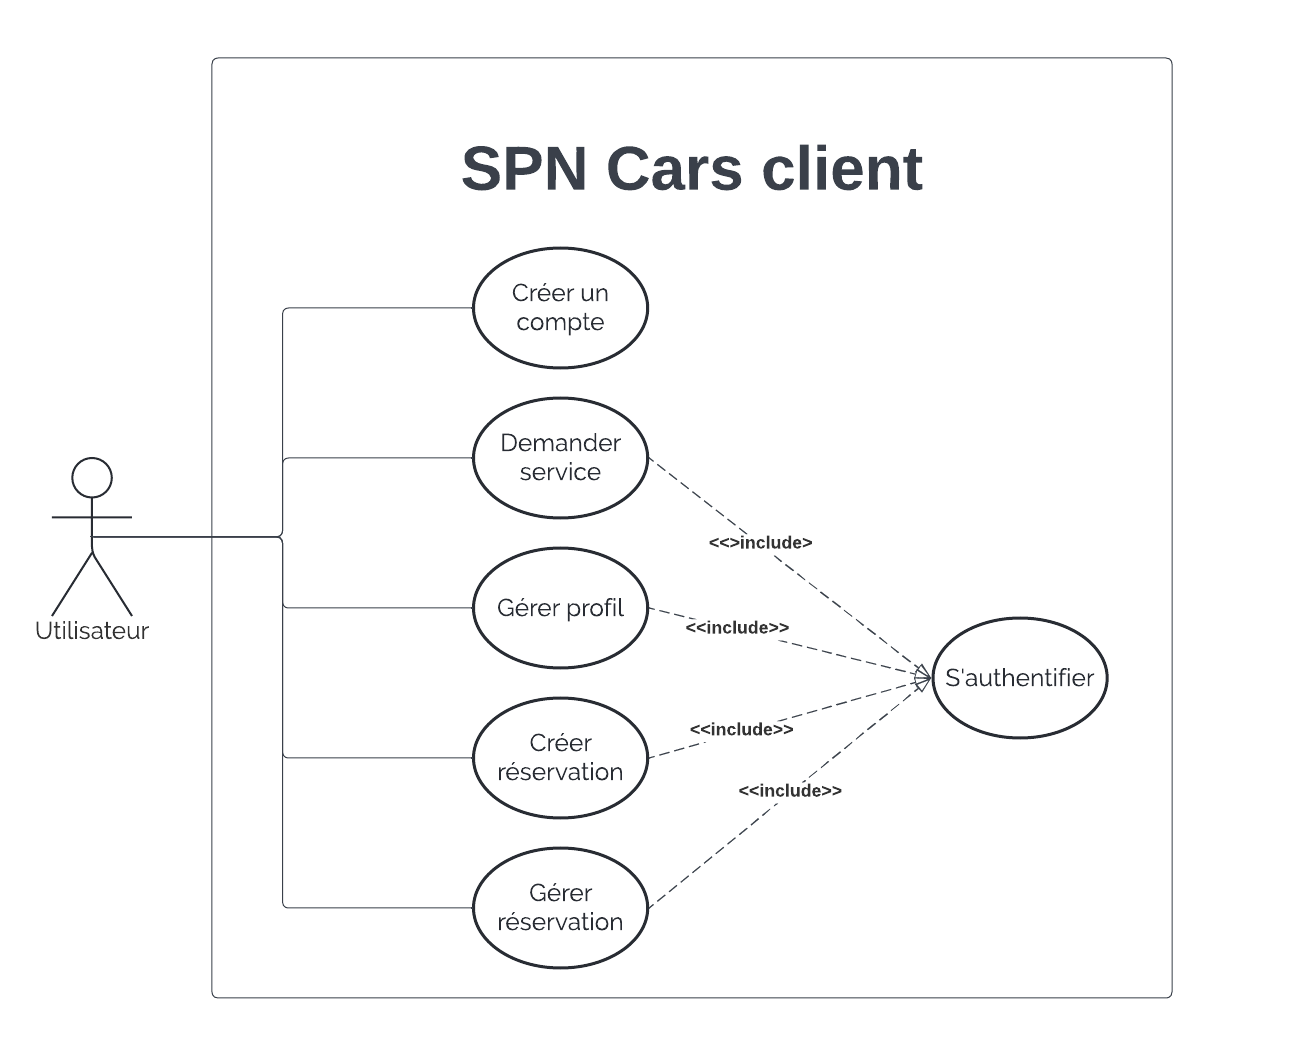
\includegraphics[height=0.5\textheight]{uml/use_cases.png}
    \vspace{1cm}
    \captionsetup{justification=centering}
    \caption{Diagramme de cas d'utilisation généralisé}
    \label{fig:use_case_diag}
\end{figure}
\subsection{Création de compte}
Avant d'utiliser les services offerts par l'application par l'application SPN Cars, l'utilisateur doit créer un compte.
\begin{table}[H]
    \begin{center}
        \begin{tabularx}{\textwidth} {
                | >{\centering\arraybackslash}X
                | >{\centering\arraybackslash}X
                | >{\centering\arraybackslash}X |}
            \hline
            Cas d'utilisation  & Scénario optimal        & Scénario d'exception                                                          \\
            \hline
            Création de compte & Compte créé avec succés & Compte non créé suite à une erreur : Email déjà utilisé / Serveur hors ligne. \\
            \hline
        \end{tabularx}
        \captionsetup{justification=centering}
        \caption{Scénario d'utilisation : Création de compte}
        \label{tab:register_scenario}
    \end{center}
\end{table}
\vspace{1cm}
\begin{figure}[H]
    \centering
    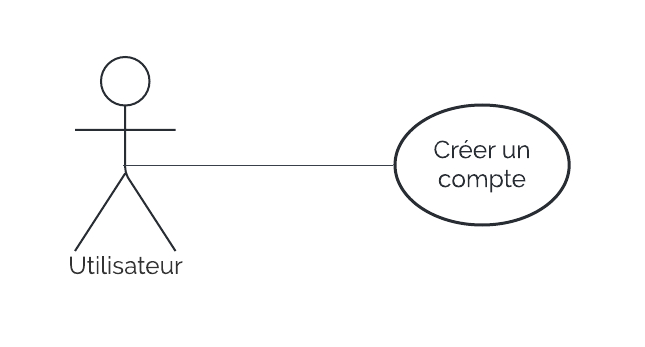
\includegraphics[width = \textwidth]{uml/register_use_case.png}
    \captionsetup{justification = centering}
    \caption{Diagramme de cas d'utilisation spécifique: Création de compte.}
    \label{fig:register_use_case}
\end{figure}
\subsection{Authentification}
Pour accéder aux différents services de l'application SPN-Cars, l'utilisateur doit s'authentifier. Cette étape consiste à vérifier les information de l'utilisateur dans la base de données.
\begin{table}[H]
    \begin{center}
        \begin{tabularx}{\textwidth} {
                | >{\centering\arraybackslash}X
                | >{\centering\arraybackslash}X
                | >{\centering\arraybackslash}X |}
            \hline
            Cas d'utilisation & Scénario optimal                                                      & Scénario d'exception                                                                                                                                     \\
            \hline
            Authentification  & Authentification réussie et un token d'authentification est retourné. & Retour d'un erreur : Coordonnées incorrectes / méthode de connexion incorrecte (Ex:Utilisation email et mot de passe au lieu du bouton Google ou Apple). \\
            \hline
        \end{tabularx}
        \captionsetup{justification=centering}
        \caption{Scénario d'utilisation : Authentification}
        \label{tab:login_scenario}
    \end{center}
\end{table}
\vspace{1cm}
\begin{figure}[H]
    \centering
    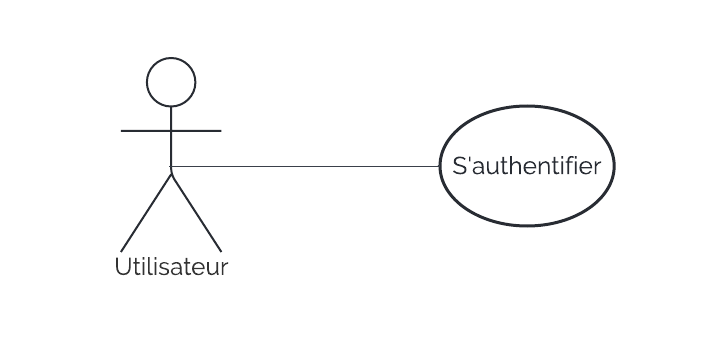
\includegraphics[width=\textwidth]{uml/login_use_case.png}
    \vspace{1cm}
    \captionsetup{justification=centering}
    \caption{Diagramme de cas d'utilisation spécifique: Authentification.}
    \label{fig:use_case_login}
\end{figure}
\subsection{Gérer profil}
L'utilisateur peut gérer son profil : Il peut changer sa photo de profil et ses informations personnelles.
\begin{table}[H]
    \begin{center}
        \begin{tabularx}{\textwidth} {
                | >{\centering\arraybackslash}X
                | >{\centering\arraybackslash}X
                | >{\centering\arraybackslash}X |}
            \hline
            Cas d'utilisation                     & Scénario optimal                  & Scénario d'exception                                             \\
            \hline
            Changement de photo de profil         & Photo ajoutée avec succés         & Photo non ajoutés : Connexion au serveur échouée.                \\
            \hline
            Changer les informations personnelles & Informations changées avec succés & Informations non changées: Erreur de connexion vers le serveur . \\
            \hline
        \end{tabularx}
        \captionsetup{justification=centering}
        \caption{Scénario d'utilisation : Création de compte}
        \label{tab:profile_update_scenario}
    \end{center}
\end{table}
\begin{figure}[H]
    \centering
    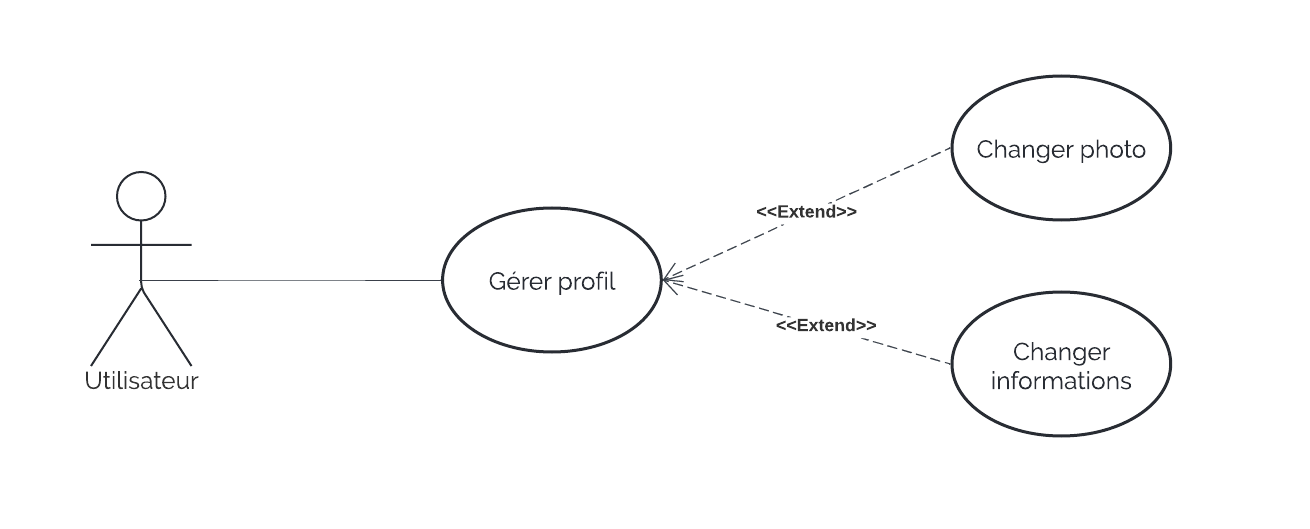
\includegraphics[width=\textwidth]{uml/profile_use_case.png}
    \vspace{1cm}
    \captionsetup{justification=centering}
    \caption{Diagramme de cas d'utilisation spécifique: Gestion de profil.}
    \label{fig:use_case_manage_profile}
\end{figure}
\subsection{Créer réservation}
Pour créer sa réservation, l'utilisateur doit louer une voiture, effectuer un paiement et signer le contrat numérique de location.\\
\begin{table}[H]
    \begin{center}
        \begin{tabularx}{\textwidth} {
                | >{\centering\arraybackslash}X
                | >{\centering\arraybackslash}X
                | >{\centering\arraybackslash}X |}
            \hline
            Cas d'utilisation  & Scénario optimal               & Scénario d'exception                                                         \\
            \hline
            Louer une voiture  & Voiture louée avec succés.     & Voiture non louée : Voiture non disponible / Erreur de connexion.            \\
            \hline
            Effectuer paiement & Paiement effectué avec succés. & Paiement non effectué : Solde insuffisant, Service de paiement indisponible. \\
            \hline
            Signer contrat     & Contrat signé avec succés.     & Contrat non signé par l'utilisateur.                                         \\
            \hline
        \end{tabularx}
        \captionsetup{justification=centering}
        \caption{Scénario d'utilisation : Créer une réservation}
        \label{tab:reservation_scenario}
    \end{center}
\end{table}
\begin{figure}[H]
    \centering
    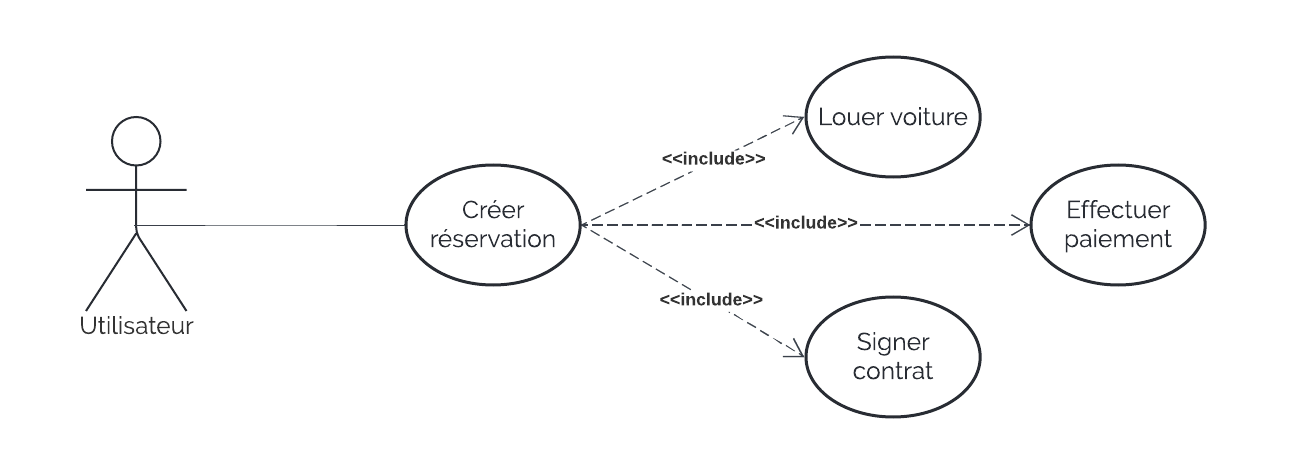
\includegraphics[width=\textwidth]{uml/reservation_use_case.png}
    \vspace{1cm}
    \captionsetup{justification=centering}
    \caption{Diagramme de cas d'utilisation spécifique: Créer réservation.}
    \label{fig:use_case_create_res}
\end{figure}
\subsection{Gérer réservation}
L'utilisateur peut gérer sa réservation, il peut suivre la position de la voiture louée en temps réel, et il peut aussi annuler sa réservation.
\begin{table}[H]
    \begin{center}
        \begin{tabularx}{\textwidth} {
                | >{\centering\arraybackslash}X
                | >{\centering\arraybackslash}X
                | >{\centering\arraybackslash}X |}
            \hline
            Cas d'utilisation   & Scénario optimal                 & Scénario d'exception                                                            \\
            \hline
            Suivi véhicules     & Véhicule suivie.                 & Véhicule non suivie : Signal GPS faible / problème de connexion avec chauffeur. \\
            \hline
            Annuler réservation & Réservation annulée avec succés. & Réservation non trouvée / Problème de connexion avec le serveur.                \\
            \hline
        \end{tabularx}
        \captionsetup{justification=centering}
        \caption{Scénario d'utilisation : Gérer une réservation}
        \label{tab:manage_reservation_scenario}
    \end{center}
\end{table}
\begin{figure}[H]
    \centering
    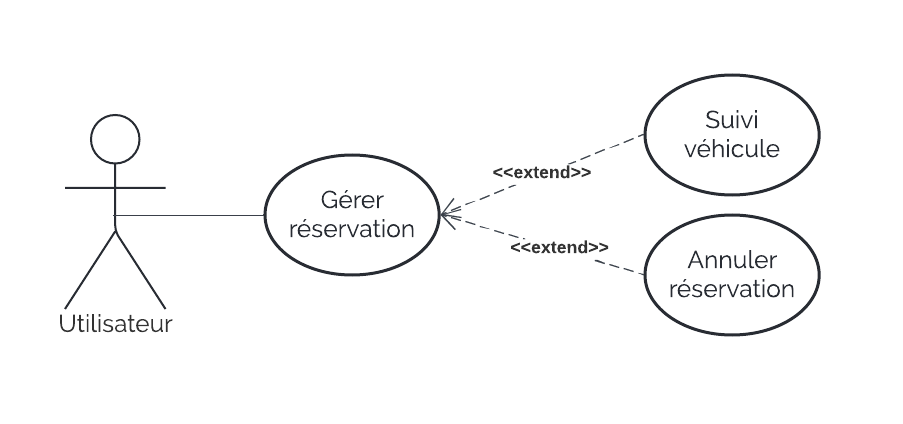
\includegraphics[width=\textwidth]{uml/manage_res_use_case.png}
    \vspace{1cm}
    \captionsetup{justification=centering}
    \caption{Diagramme de cas d'utilisation spécifique: Gérer réservation.}
    \label{fig:use_case_manage_res}
\end{figure}


\subsection{Diagramme de classes}
\begin{figure}[H]
    \centering
    \rotatebox[origin=c]{-90}{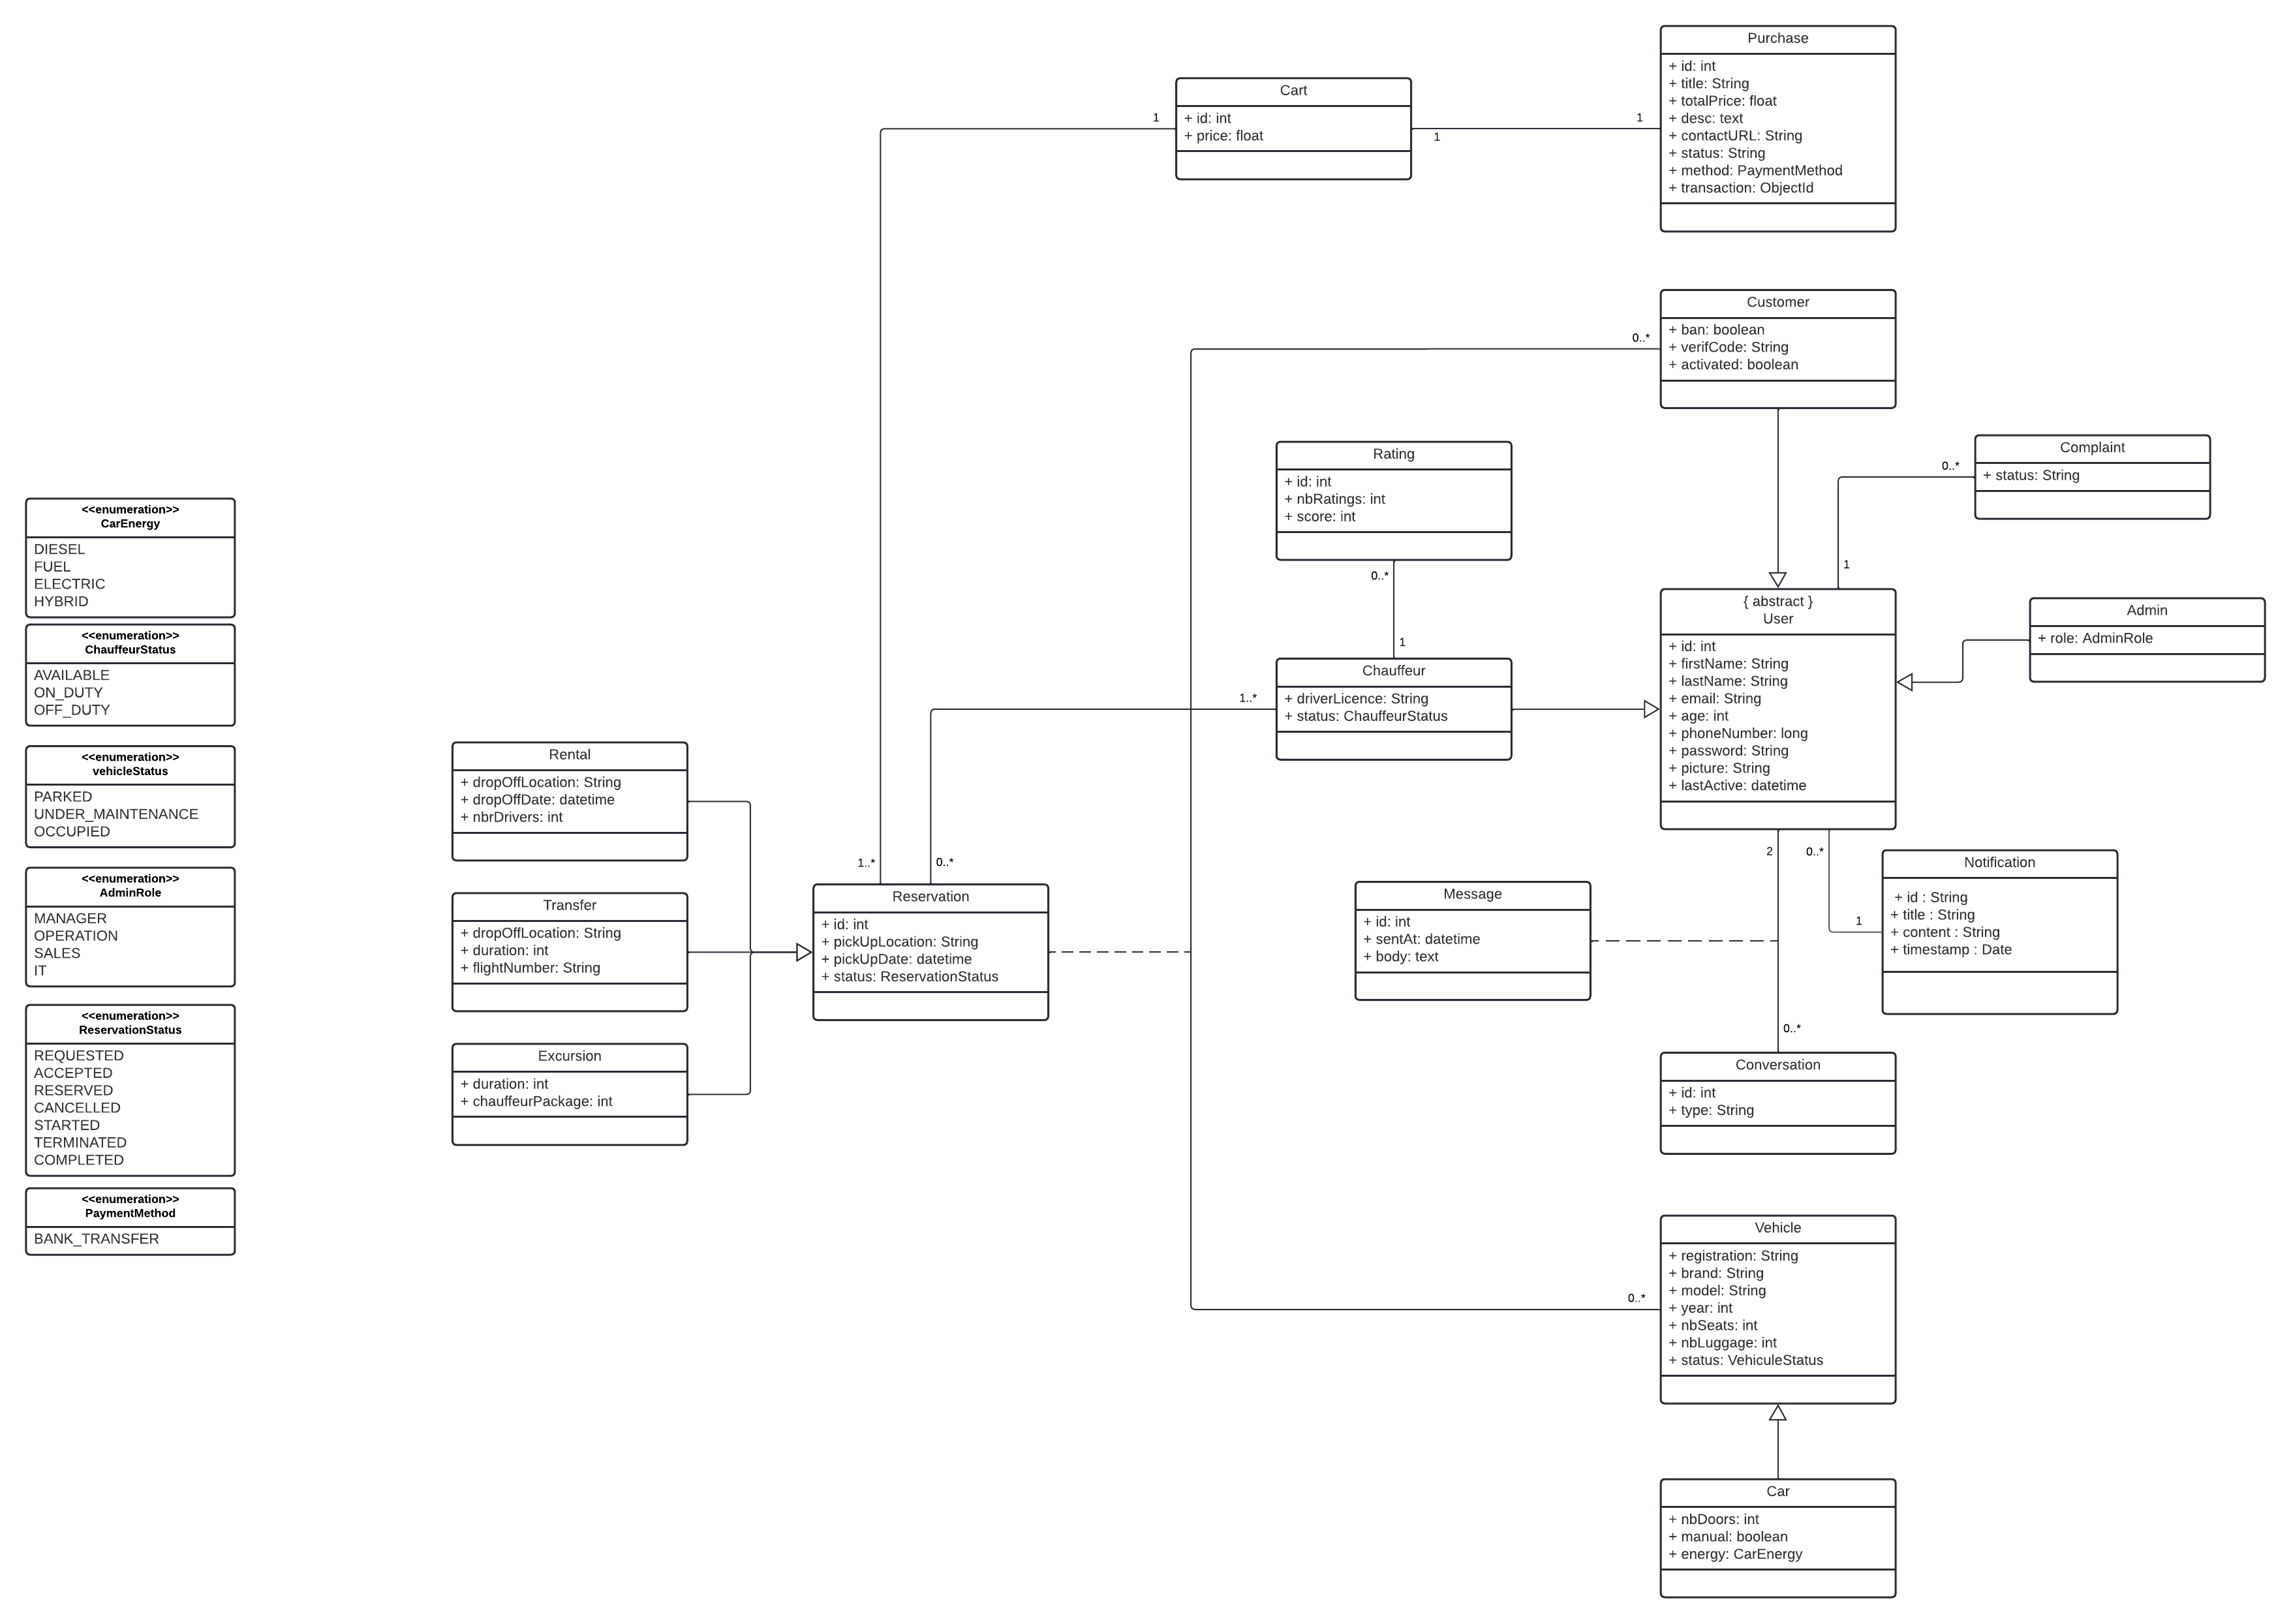
\includegraphics[width=0.9\textheight,height=\textwidth]{uml/class_diag.png}}
    \vspace{1cm}
    \captionsetup{justification=centering}

    \caption{Diagramme de classe}
    \label{fig:class_diag}
\end{figure}
\clearpage
\subsection{Diagrammes de séquences}
Les diagrammes de séquences sont le moyen qui permettent de décrire d'une manière détaillée les différents cas d'utilisation
\subsubsection{Création de compte}
\begin{figure}[H]
    \centering
    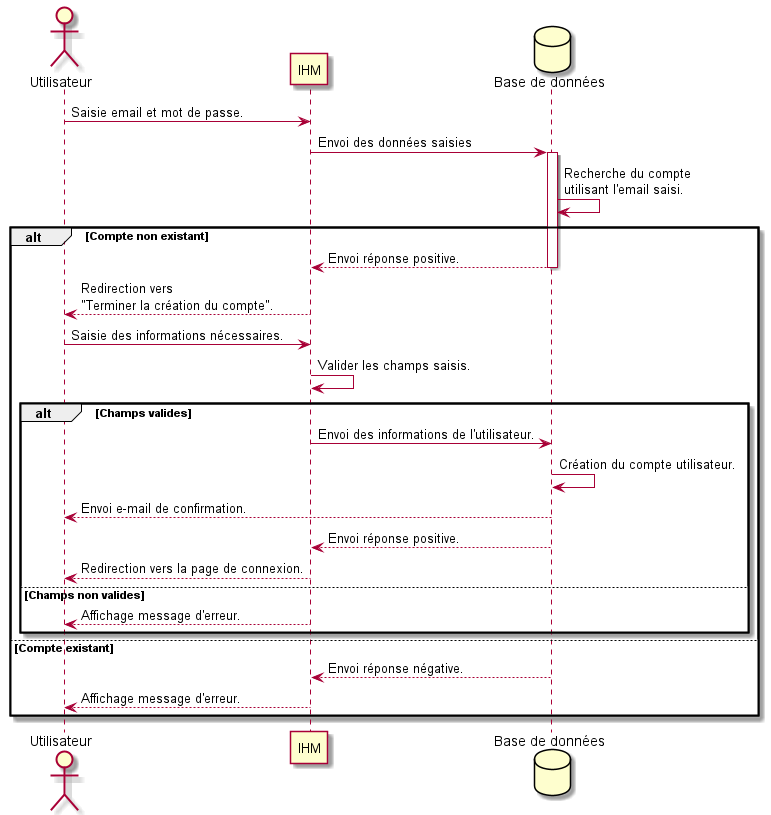
\includegraphics[width = \textwidth]{uml/register_email.png}
    \vspace{1cm}
    \captionsetup{justification=centering}

    \caption{Diagramme de séquence : Création de compte avec E-mail et mot de passe.}
    \label{fig:seq_register_email}
\end{figure}
\begin{figure}[H]
    \centering
    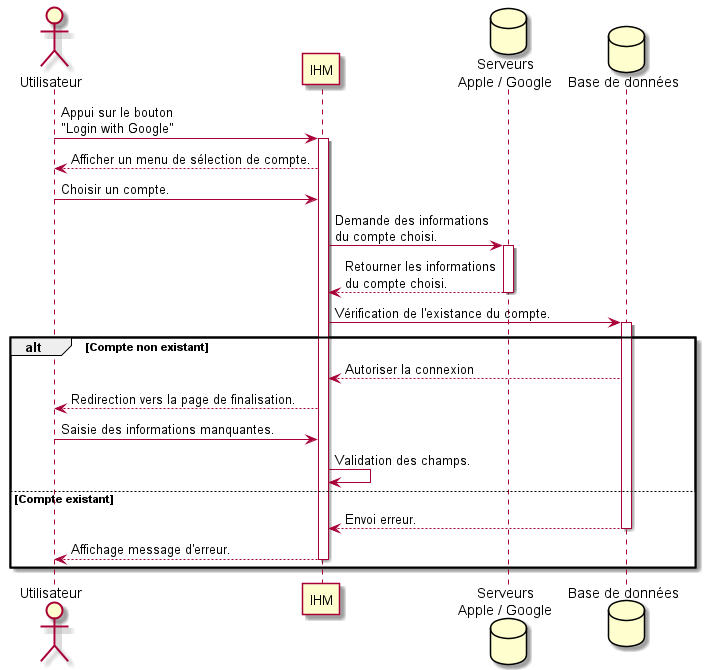
\includegraphics[width = \textwidth]{uml/apple_google.png}
    \vspace{1cm}
    \captionsetup{justification=centering}

    \caption{Diagramme de séquence : Création de compte avec un compte Google / Apple.}
    \label{fig:seq_register_apple_google}
\end{figure}
\subsubsection{Authentification}
\begin{center}
    \begin{figure}[H]
        \centering
        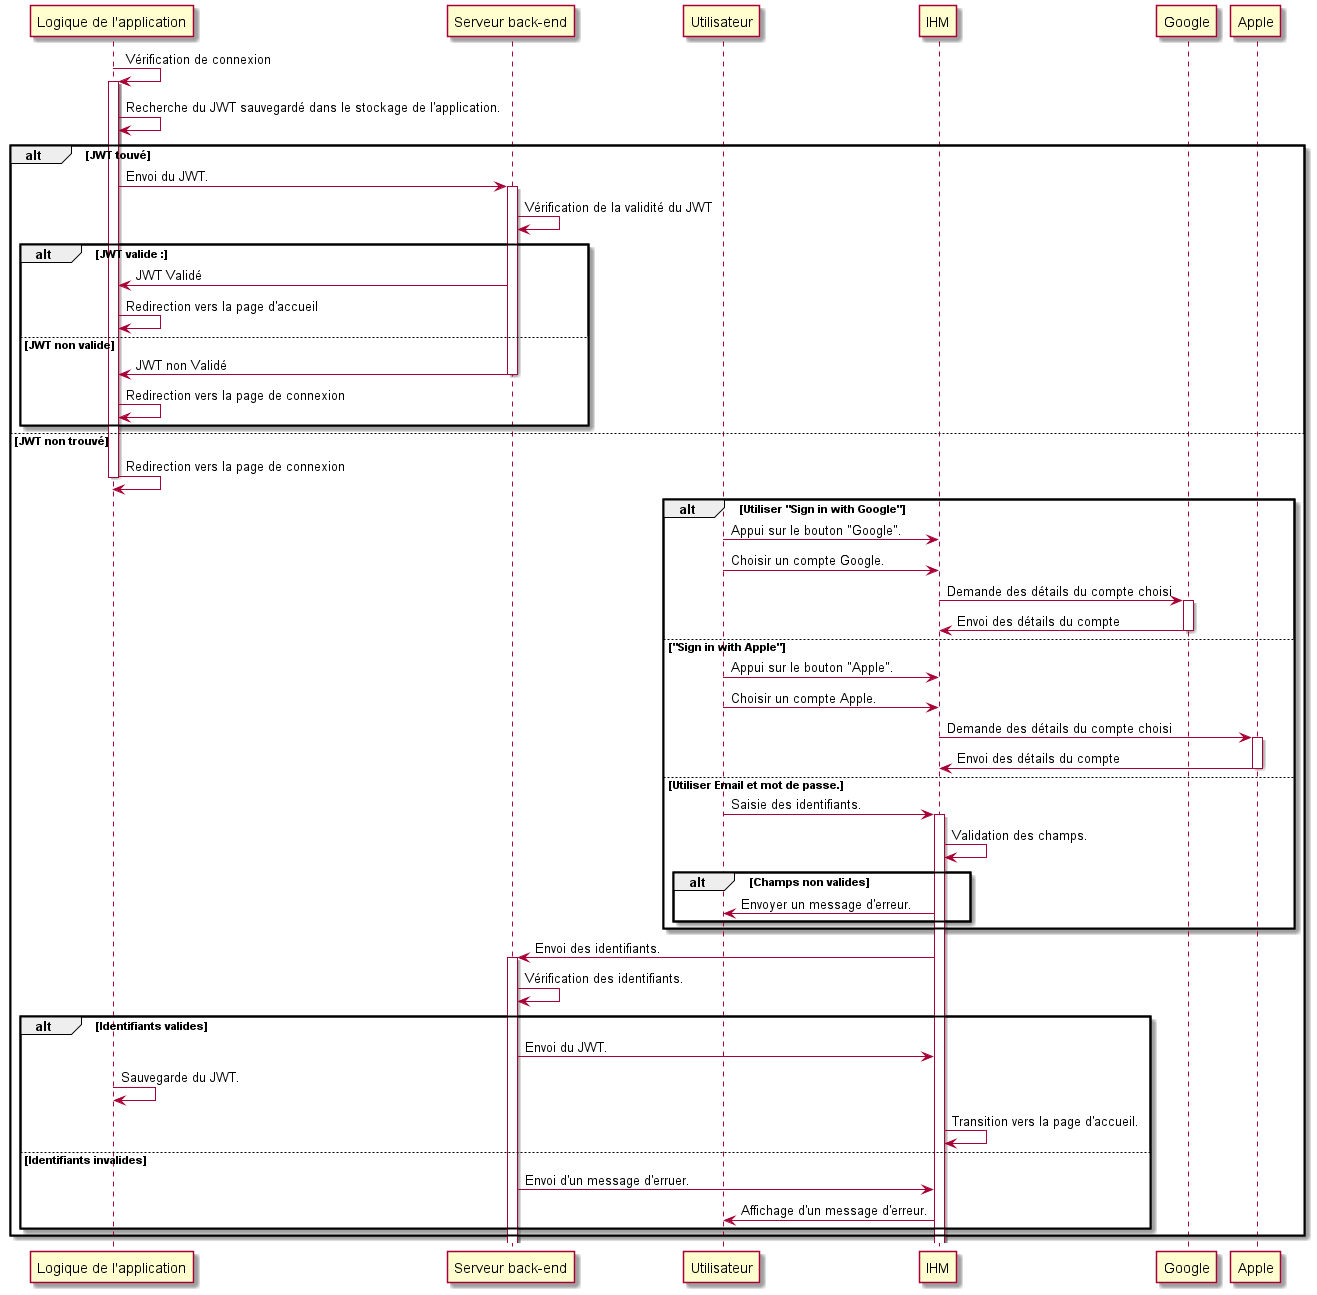
\includegraphics[width = \textwidth]{uml/Authentification.png}
        \vspace{1cm}
        \captionsetup{justification=centering}

        \caption{Diagramme de séquences: Authentification.}
        \label{fig:seq_auth}
    \end{figure}
\end{center}
\subsubsection{Page d'accueil}
\begin{figure}[H]
    \centering
    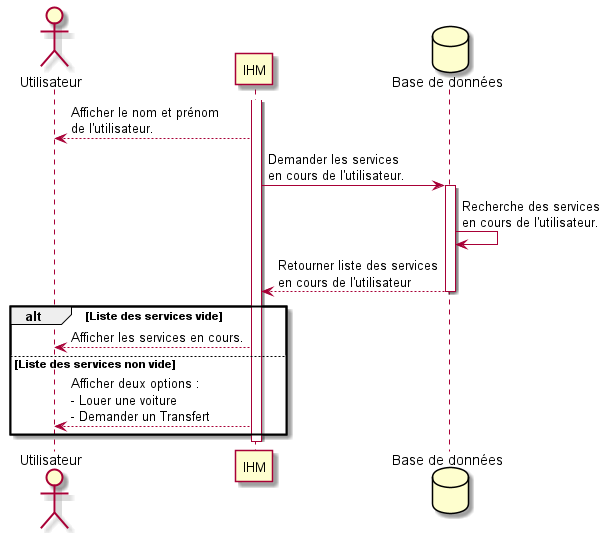
\includegraphics[width=\textwidth]{uml/home.png}
    \vspace{1cm}
    \caption{Diagramme de séquences : Page d'accueil.}
    \label{fig:seq_home}
\end{figure}
% \subsubsection{Gestion de profil}
\subsubsection{Demander un service}
\begin{figure}[H]
    \centering
    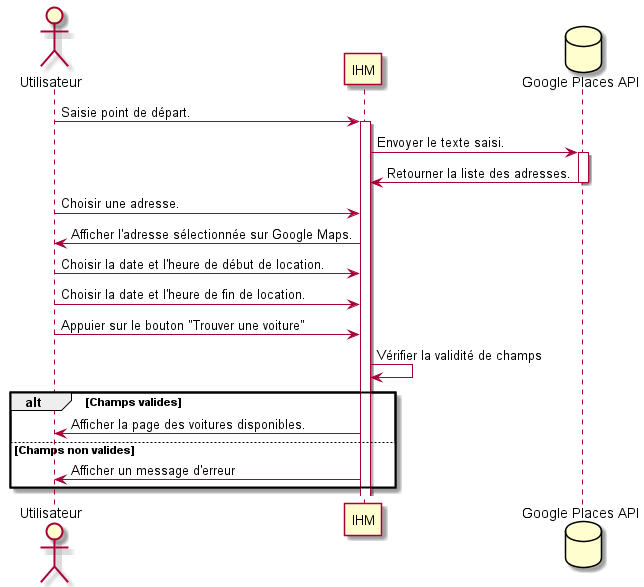
\includegraphics[width = \textwidth]{uml/rent a car.png}
    \vspace{1cm}
    \captionsetup{justification=centering}

    \caption{Diagramme de séquences: Demander une location.}
    \label{fig:seq_location}
\end{figure}
\vspace{1cm}
\begin{figure}[H]
    \centering
    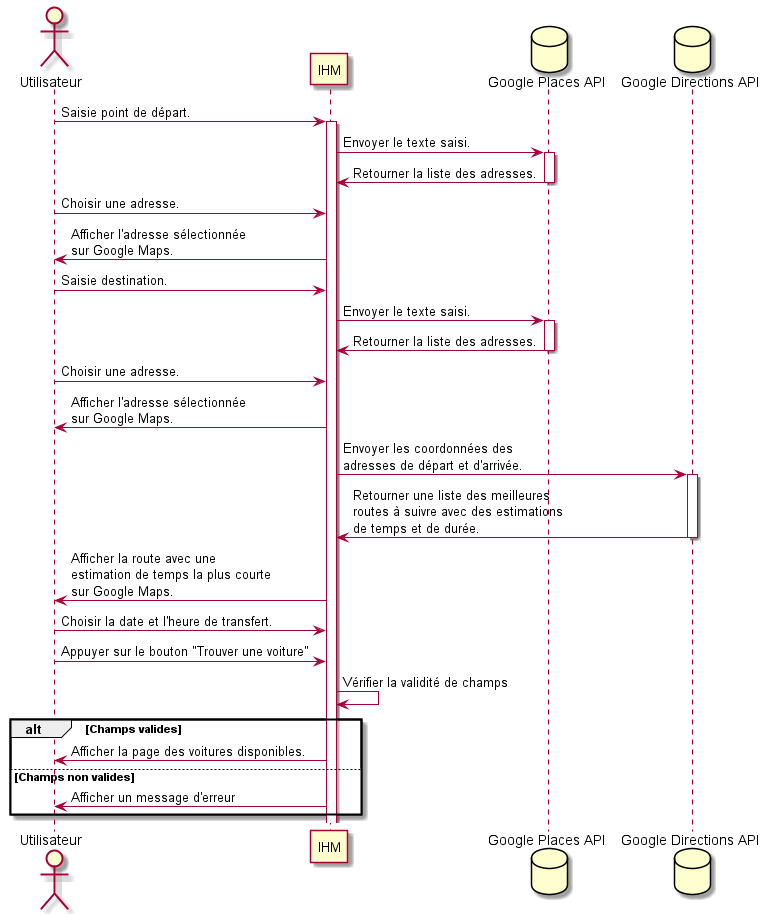
\includegraphics[width = \textwidth]{uml/transfert.png}
    \vspace{1cm}
    \captionsetup{justification=centering}

    \caption{Diagramme de séquences: Demander un transfert.}
    \label{fig:seq_transfert}
\end{figure}
\subsubsection{Affichage des voitures disponibles}
\begin{figure}[H]
    \centering
    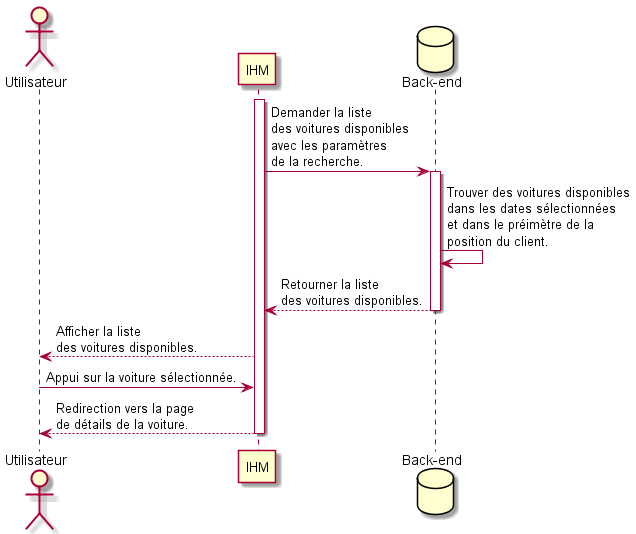
\includegraphics[width = \textwidth]{uml/choisir voiture.png}
    \vspace{1cm}
    \captionsetup{justification=centering}

    \caption{Diagramme de séquences : Choisir une voiture}
    \label{fig:seq_car_select}
\end{figure}
\subsubsection{Signature numérique de contrat de location}
\begin{figure}[H]
    \centering
    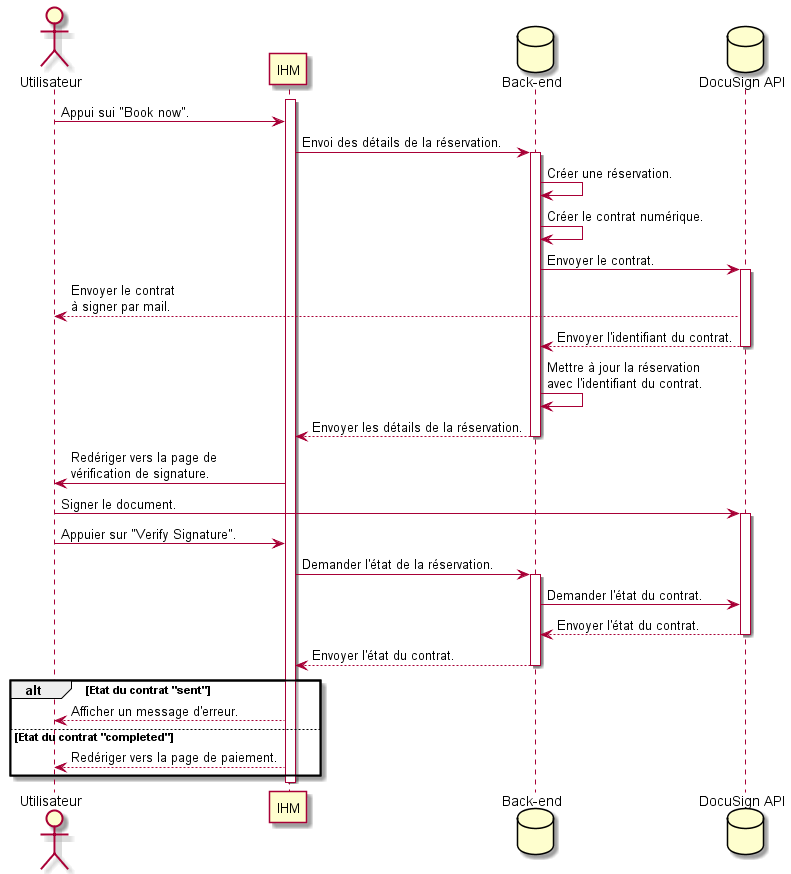
\includegraphics[width = \textwidth]{uml/docusign.png}
    \captionsetup{justification=centering}
    \caption{Diagramme de séquences : Envoi du contrat de location.}
    \label{fig:seq_location_contract}
\end{figure}
\subsubsection{Paiement en ligne}
\begin{figure}[H]
    \centering
    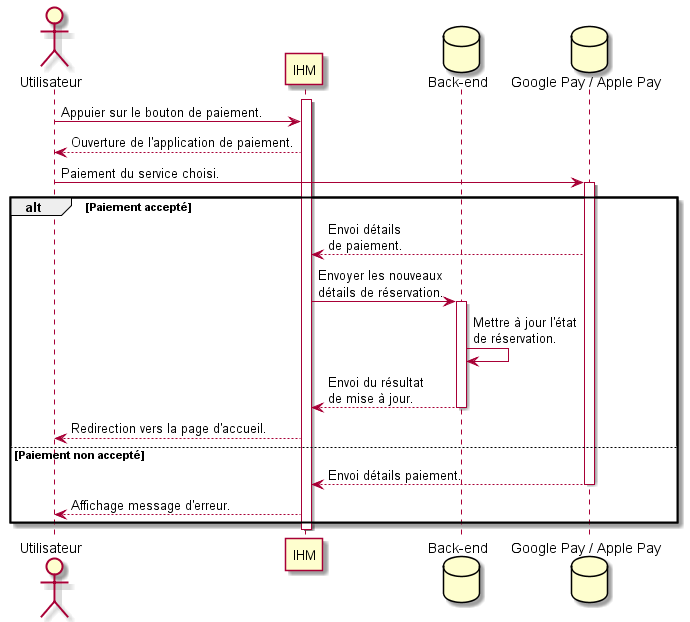
\includegraphics[width = \textwidth]{uml/payment.png}
    \captionsetup{justification=centering}
    \caption{Diagramme de séquences: Paiement des services.}
    \label{fig:seq_payment}
\end{figure}
\subsubsection{Localiser une voiture}
\section{UI/UX Design}
Avant de passer au développement de l'application, il faut créer d'abord les prototypes des interfaces utilisateur. \\
\noindent Cette étape est nécessaire pour tester plusieurs approches dans les interfaces de l'application, s'assurer d'offrir une expérience optimale pour l'utilisateur. \\
\noindent Suite à une collaboration avec l'équipe de design UI/UX, les interfaces suivantes ont été créées.
\vspace{1cm}
\begin{multicols}{2}
    \begin{figure}[H]
        \centering
        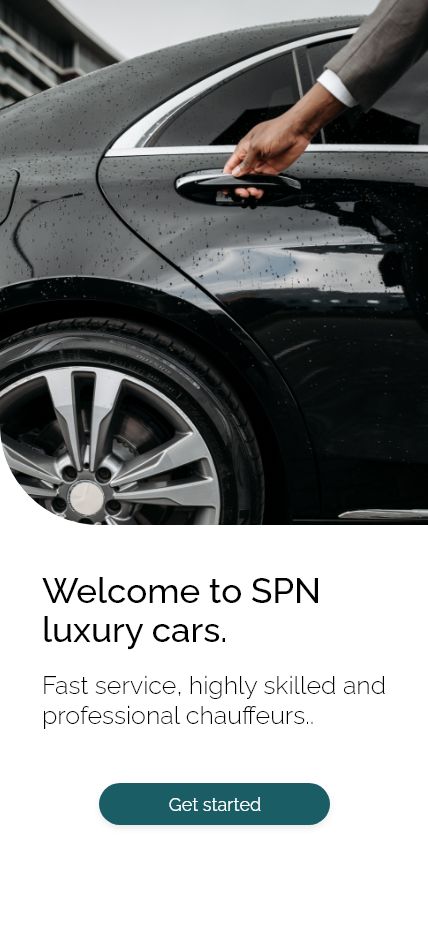
\includegraphics[width=0.25\textwidth]{ui_screenshots/Guide.png}
        \vspace{1cm}
        \captionsetup{justification=centering}

        \caption{Première page.}
        \label{fig:start_page}
    \end{figure}
    \begin{figure}[H]
        \centering
        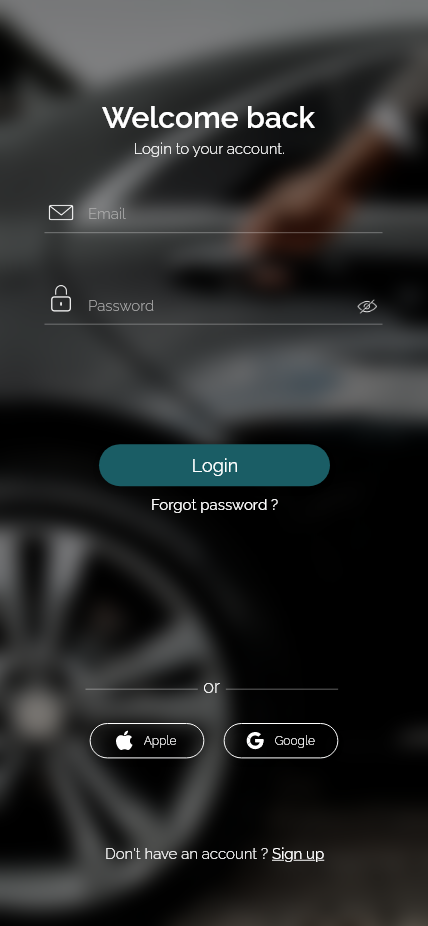
\includegraphics[width=0.25\textwidth]{ui_screenshots/sign in.png}
        \vspace{1cm}
        \captionsetup{justification=centering}

        \caption{Page de connexion.}
        \label{fig:sign_in_page}
    \end{figure}
\end{multicols}
% \newpage
\begin{multicols}{2}
    \begin{figure}[H]
        \centering
        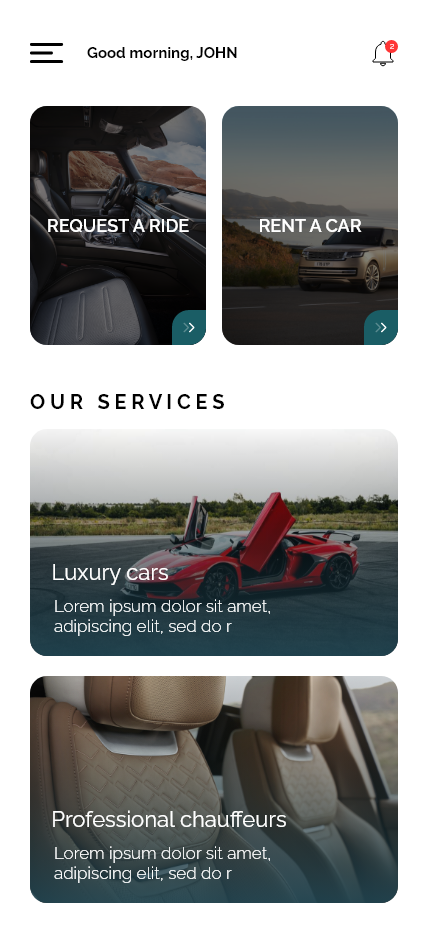
\includegraphics[width=0.25\textwidth]{ui_screenshots/No Active trip.png}
        \vspace{1cm}
        \captionsetup{justification=centering}

        \caption{\centering Page d'accueil.}
        \label{fig:no_active_trip}
    \end{figure}
    \begin{figure}[H]
        \centering
        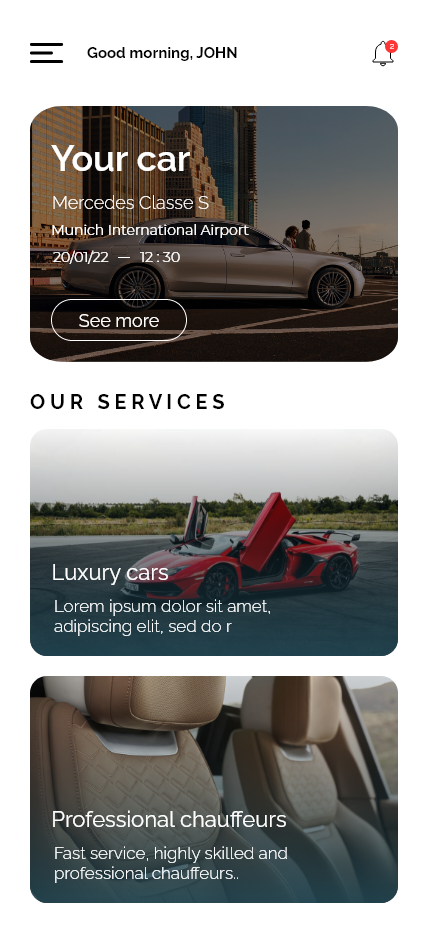
\includegraphics[width=0.25\textwidth]{ui_screenshots/Active trip.png}
        \vspace{1cm}
        \captionsetup{justification=centering}

        \caption{\centering Page d'accueil lors d'un transfert en cours.}
        \label{fig:active_trip}
    \end{figure}
\end{multicols}
\clearpage
\begin{multicols}{2}
    \begin{figure}[H]
        \centering
        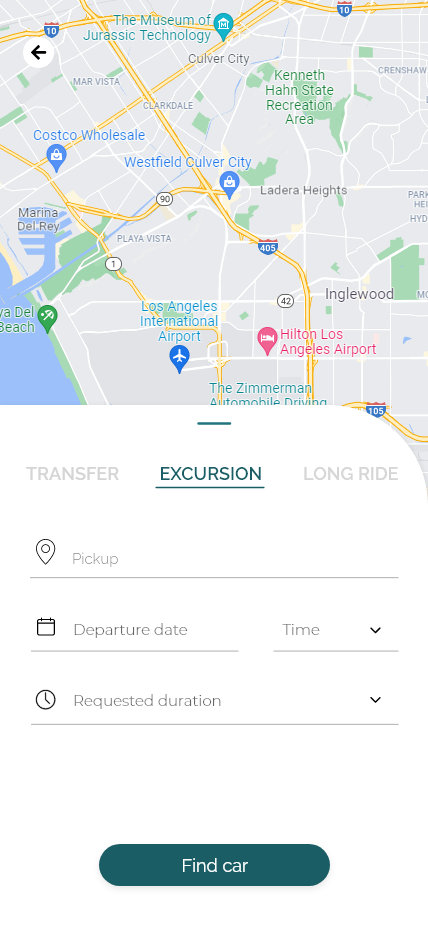
\includegraphics[width=0.25\textwidth]{ui_screenshots/Excursion.png}
        \vspace{1cm}
        \captionsetup{justification=centering}

        \caption{\centering Sélection de type de transfert.}
        \label{fig:trip_select}
    \end{figure}
    \begin{figure}[H]
        \centering
        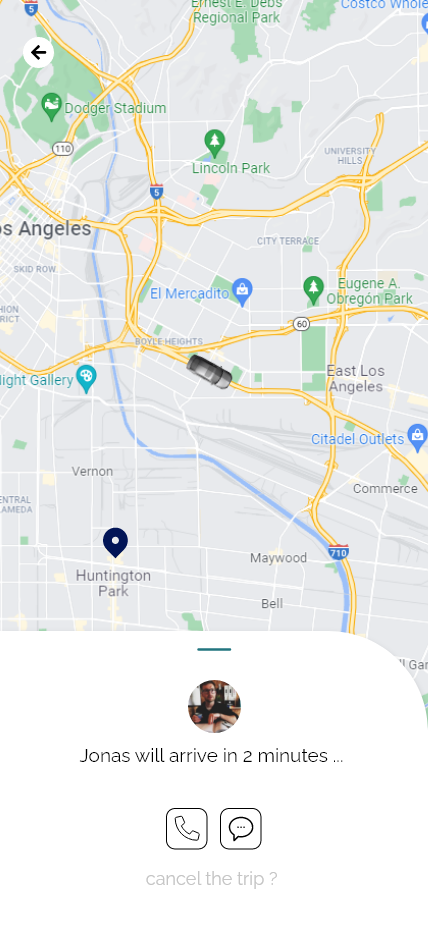
\includegraphics[width=0.25\textwidth]{ui_screenshots/Map view.png}
        \vspace{1cm}
        \captionsetup{justification=centering}

        \caption{\centering Suivi de la position actuelle du chauffeur avec la voiture.}
        \label{fig:follow_driver}
    \end{figure}
\end{multicols}
\begin{multicols}{2}
    \begin{figure}[H]
        \centering
        \includegraphics[width=0.25\textwidth]{ui_screenshots/Available cars – 1.png}
        \vspace{1cm}
        \captionsetup{justification=centering}

        \caption{\centering Liste des voitures disponibles.}
        \label{fig:available_cars}
    \end{figure}
    \begin{figure}[H]
        \centering
        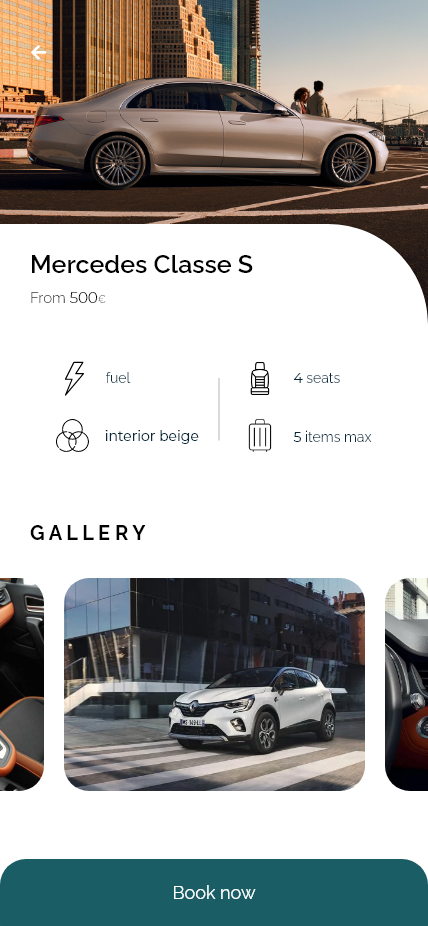
\includegraphics[width=0.25\textwidth]{ui_screenshots/Car details.png}
        \vspace{1cm}
        \captionsetup{justification=centering}

        \caption{\centering Détails de la voiture sélectionnée.}
        \label{fig:car_details}
    \end{figure}
\end{multicols}
\vspace{1cm}
\begin{figure}[H]
    \centering
    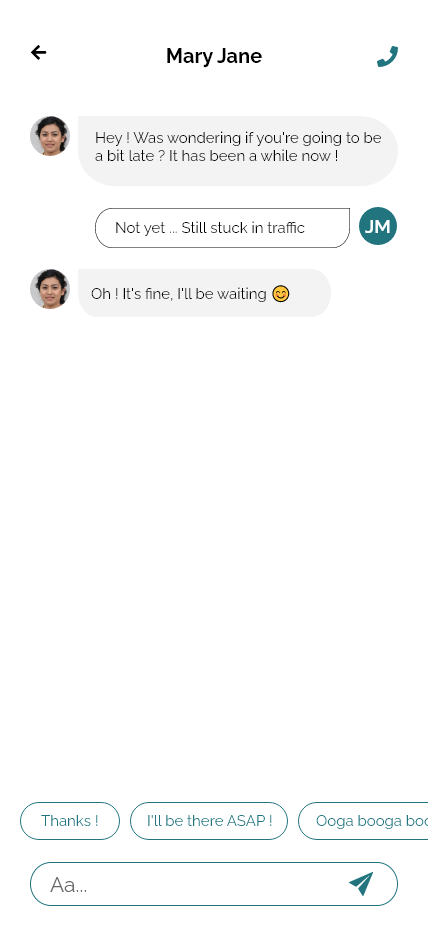
\includegraphics[width=0.25\textwidth]{ui_screenshots/DMs.png}
    \vspace{1cm}
    \caption{\centering Messagerie instantanée avec le chauffeur.}
    \label{fig:dms}
\end{figure}
\section{Conclusion}
A travers ce chapitre, on a établi la conception de l'application SPN-Cars: On a dégager les besoins fonctionnels et non fonctionnels, qui, à travers eux on a pu créer les diagrammes de cas d'utilisation, les diagrammes de classes, et les diagrammes de séquences. Suite au développement de ces diagrammes, on est passé vers l'étape de conception des interfaces utilisateur. Toutes ces différentes étapes permettront de choisir les technologies et outils qui seront utilisés pour la création de cette application, qui seront présentés dans le prochain chapitre.